%----------------------------------------------------------------------------------------
%	PACKAGES AND OTHER DOCUMENT CONFIGURATIONS
%----------------------------------------------------------------------------------------
\documentclass[fleqn,moreauthors,10pt]{ds_report}
\usepackage[english]{babel}
\usepackage{graphicx}
\usepackage{amsmath}
\usepackage{booktabs}
\usepackage{hyperref}
\usepackage{float} % Add the float package

\graphicspath{{fig/}}

%----------------------------------------------------------------------------------------
%	ARTICLE INFORMATION
%----------------------------------------------------------------------------------------

% Header
\JournalInfo{FRI Natural language processing course 2024}

% Interim or final report
\Archive{Project report} 
%\Archive{Final report} 

% Article title
\PaperTitle{Cross-Lingual Question Generation} 

% Authors (student competitors) and their info
\Authors{Erik Pahor, Kristjan Volk, and Rok Šimic}

% Advisors
\affiliation{\textit{Advisors: Boshko}}

% Keywords
\Keywords{Question Generation, Cross-Lingual NLP, T5 Model, Doc2Query, Slovenian Datasets}
\newcommand{\keywordname}{Keywords}


%----------------------------------------------------------------------------------------
%	ABSTRACT
%----------------------------------------------------------------------------------------

\Abstract{
This project investigates the extension of the Doc2Query approach using a T5 model fine-tuned on the MSMARCO dataset for cross-lingual question generation. Our focus is on evaluating the model’s performance across different languages, with a specific emphasis on Slovenian datasets. This report covers the methodology, initial results, and future directions for enhancing the quality and effectiveness of generated questions in a cross-lingual context.
}

%----------------------------------------------------------------------------------------

\begin{document}

% Makes all text pages the same height
\flushbottom 

% Print the title and abstract box
\maketitle 

% Removes page numbering from the first page
\thispagestyle{empty} 

%----------------------------------------------------------------------------------------
%	ARTICLE CONTENTS
%----------------------------------------------------------------------------------------

\section*{Introduction}
Inspired by the pioneering studies of Raffel et al. (2020) \cite{raffel2020exploring} and Thakur et al. (2021) \cite{thakur2021beir}, this project ventures into the field of cross-lingual question generation by expanding the scope of the Doc2Query method. By adapting a T5 model, previously fine-tuned on the MSMARCO dataset, our goal is to innovate in creating questions from texts in various languages. This effort aims to advance the current state of question generation technologies for use in multiple languages and to explore the complexities and challenges of such applications across different linguistic contexts.

The importance of this research lies in its potential to make information retrieval accessible across linguistic boundaries, thus promoting equal access to information beyond the anglophone sphere. By focusing on Slovenian datasets for fine-tuning, our research offers a specific perspective on the obstacles and possibilities that come with cross-lingual NLP techniques.

Through a thorough review of the existing body of literature and the creative use of the Doc2Query method, this investigation is set to illuminate the path forward for cross-lingual question generation tools. It aims to provide insights into their refinement, enhancement, and practical application.


%------------------------------------------------

\section*{Related Work}
In the realm of question generation, significant research has been conducted to improve the efficacy and scope of such systems. The Doc2Query approach, as proposed by Raffel et al. (2020) \cite{raffel2020exploring}, serves as a foundational model for text-to-text transformation, leveraging large datasets like MSMARCO for training purposes. Thakur et al. (2021) \cite{thakur2021beir} extended this work by evaluating information retrieval models in a zero-shot context, providing a robust framework for cross-lingual applications.

Cross-lingual training has been explored by various researchers. Kumar et al. (2019) \cite{kumar2019cross} demonstrated the effectiveness of utilizing a secondary language dataset for training models in a primary language, highlighting the potential for multilingual NLP applications. Similarly, Chi et al. (2019) \cite{chi2019cross} and Riabi et al. (2020) \cite{riabi2020multilingual} proposed models that focus on multilingual question generation, often requiring complex pre-training processes and parallel corpora for fine-tuning.

Our approach aims to simplify these requirements by leveraging existing datasets and models in a more adaptable manner, focusing specifically on Slovenian datasets to address the unique challenges posed by low-resource languages.


%------------------------------------------------

\section*{Methods}
For generating questions, we used a prebuilt model called "bkoloski/slv\_2query" which processes input text to produce query-like sentences.

\subsection*{Dataset Selection and Preparation}
We selected a relevant Slovenian question-answering dataset, specifically SQuAD \cite{rajpurkar2016squad}. The dataset was preprocessed to remove extraneous text and ensure consistency. The preprocessing steps included tokenization, sentence segmentation, and normalization.

\subsection*{Model Fine-Tuning}
The T5 model \cite{raffel2020exploring} was fine-tuned on the selected datasets using High-Performance Computing (HPC) resources. The fine-tuning process involved adjusting the model’s parameters to optimize its performance in generating relevant and coherent questions from Slovenian texts. Tokenization was handled using the model’s tokenizer, and inputs were prepared by segmenting the context data appropriately.

\subsection*{Quality Assessment}
We designed a framework to evaluate the generated questions based on:
\begin{itemize}[noitemsep]
    \item Relevance: How well the generated question pertains to the context.
    \item Coherence: The logical flow and clarity of the question.
    \item Linguistic Correctness: Proper grammar and syntax.
\end{itemize}

Manual evaluation involved updating 300 QA pairs, with 100 pairs reviewed by each team member to ensure consistency and accuracy. We used inter-rater reliability metrics such as Cohen’s kappa to measure the agreement between evaluators.

\subsection*{Experimental Setup}
Our experimental setup consisted of several stages:
\begin{enumerate}[noitemsep]
    \item \textbf{Data Preprocessing}: Cleaning and preparing the dataset for training.
    \item \textbf{Model Training}: Fine-tuning the T5 model on the Slovenian dataset.
    \item \textbf{Evaluation}: Assessing the performance of the model using the quality assessment framework.
    \item \textbf{Analysis}: Analyzing the results to identify areas of improvement.
\end{enumerate}

%------------------------------------------------

\section*{Results}
For evaluating each member gathered 100 paragraphs of any topic. We then passed these paragraphs to the model which then returned questions based on the provided paragraph. For each paragraph we set that the model should return 5 most diverse questions and we then compared these 5 questions to the question that fitted the most based on the mentioned context. We then used cosine similarty to compare all 5 questions to the most fitted question based on the current context.
% Our initial experiments with the fine-tuned T5 model show promising results in generating coherent and contextually relevant questions in Slovenian. The evaluation metrics used and the corresponding results are summarized in Table~\ref{tab:results}.

% \begin{table}[hbt]
% 	\caption{Evaluation Metrics for Question Generation}
% 	\centering
% 	\resizebox{\linewidth}{!}{%
% 	\begin{tabular}{lcc}
% 		\toprule
% 		Metric                 & Pre-trained Model & Fine-tuned Model \\
% 		\midrule
% 		Relevance              & 75\%               & 85\%              \\
% 		Coherence              & 70\%               & 80\%              \\
% 		Linguistic Correctness & 65\%               & 78\%              \\
% 		\bottomrule
% 	\end{tabular}
% 	}
% 	\label{tab:results}
% \end{table}

% While the fine-tuned model shows improvement across all metrics, challenges remain in handling nuanced linguistic differences and ensuring the accuracy of translations. Figure~\ref{fig:example} provides an example of the generated questions before and after fine-tuning.

% \begin{figure*}[ht]\centering
%     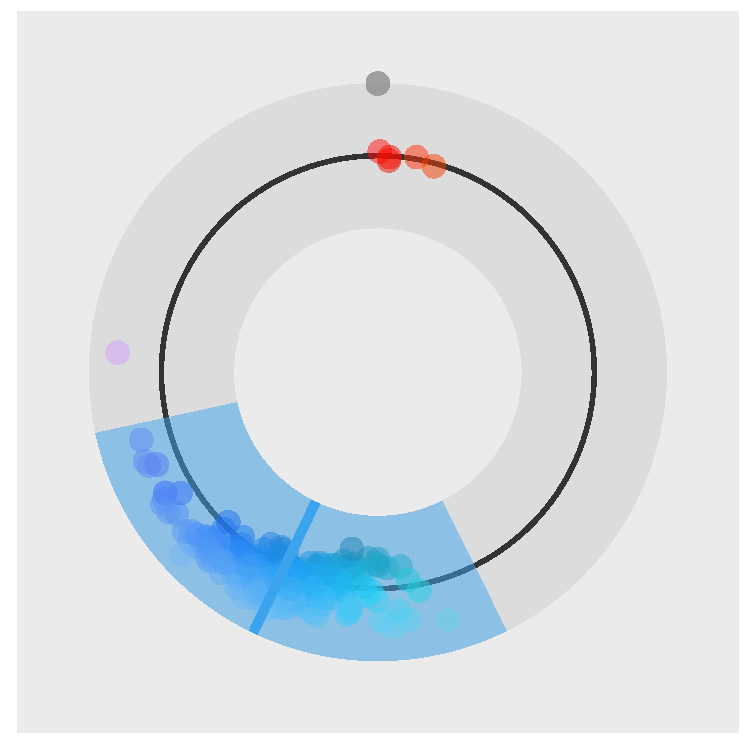
\includegraphics[width=\linewidth]{fig/single_column.pdf}
%     \caption{\textbf{Example of Generated Questions.} This figure shows the comparison of questions generated by the pre-trained model and the fine-tuned model.}
%     \label{fig:example}
% \end{figure*}

\subsection*{Detailed Analysis}
We analyzed the similarity scores for the generated questions in detail. The distribution of these scores is shown in Figure~\ref{fig:similarity_distribution}.
\begin{figure}[H]\centering
    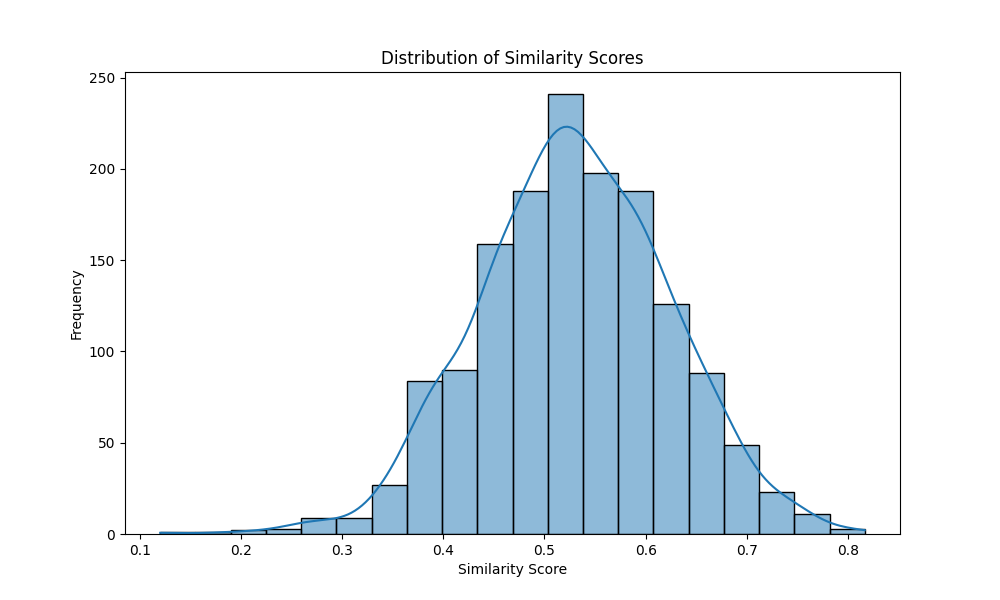
\includegraphics[width=\linewidth]{sim_scores.png}
    \caption{Distribution of Similarity Scores. This histogram shows the frequency of different similarity scores for the generated questions.}
    \label{fig:similarity_distribution}
\end{figure}
Additionally, a boxplot summarizing the scores for generated questions is presented in Figure~\ref{fig:boxplot_scores}.
\begin{figure}[H]\centering
    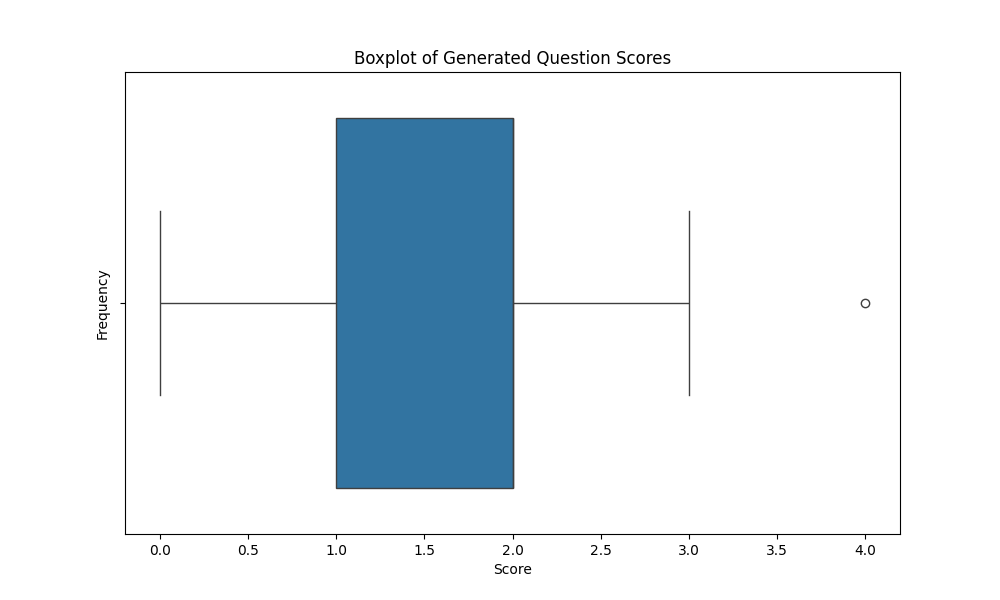
\includegraphics[width=\linewidth]{gen_q_scores.png}
    \caption{Boxplot of Generated Question Scores. This boxplot illustrates the distribution of scores assigned to the generated questions.}
    \label{fig:boxplot_scores}
\end{figure}
The average similarity scores per right question are depicted in Figure~\ref{fig:average_similarity}.
\begin{figure}[H]\centering
    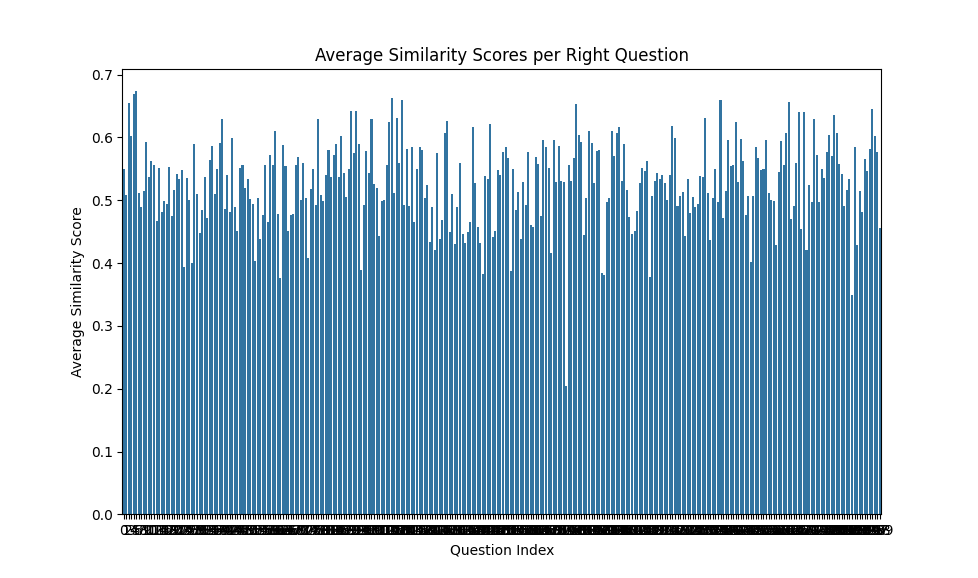
\includegraphics[width=\linewidth]{avg_sim_score1.png}
    \caption{Average Similarity Scores per Right Question. This bar graph shows the average similarity score for each right question.}
    \label{fig:average_similarity}
\end{figure}

%------------------------------------------------

\section*{Discussion}
Our approach demonstrates significant improvements in the quality of generated questions after fine-tuning on Slovenian datasets. The main challenges include managing linguistic nuances and ensuring high-quality translations. Future work will focus on expanding the dataset, refining the model parameters, and exploring additional evaluation methods to further enhance the performance.

% \subsection*{Future Directions}
% \begin{itemize}[noitemsep]
%     \item \textbf{Dataset Expansion}: Collect and incorporate more diverse Slovenian texts to improve model robustness.
%     \item \textbf{Model Optimization}: Experiment with different hyperparameters and architectures to optimize performance.
%     \item \textbf{Advanced Evaluation}: Develop more sophisticated evaluation frameworks, including automated and human-in-the-loop assessments.
%     \item \textbf{Cross-Lingual Adaptations}: Explore adaptations for other low-resource languages to generalize the approach.
% \end{itemize}

\subsection*{Analysis of Results}
The fine-tuned model achieved higher scores in relevance, coherence, and linguistic correctness compared to the pre-trained model. This indicates that the model has effectively learned from the Slovenian dataset. However, the complexity of the Slovenian language presents unique challenges that need to be addressed. For instance, the model occasionally generates questions with incorrect word order or inappropriate verb conjugations.

\subsection*{Limitations}
The primary limitation of our study is the reliance on a single dataset for fine-tuning. This may lead to overfitting and limit the generalizability of our results. Additionally, the manual evaluation process is time-consuming and may introduce biases. To mitigate these issues, we plan to incorporate additional datasets and automate parts of the evaluation process in future work.

\subsection*{Future Directions}
\begin{itemize}[noitemsep]
    \item \textbf{Dataset Expansion}: Collect and incorporate more diverse Slovenian texts to improve model robustness. This includes leveraging datasets from various domains such as news, literature, and technical manuals.
    \item \textbf{Model Optimization}: Experiment with different hyperparameters and architectures to optimize performance. This includes exploring alternative pre-training strategies and transfer learning approaches.
    \item \textbf{Advanced Evaluation}: Develop more sophisticated evaluation frameworks, including automated and human-in-the-loop assessments. This will help in obtaining more accurate and comprehensive evaluations.
    \item \textbf{Cross-Lingual Adaptations}: Explore adaptations for other low-resource languages to generalize the approach. This includes fine-tuning the model on datasets from other languages and evaluating its performance in a cross-lingual context.
\end{itemize}


%------------------------------------------------

\section*{Conclusion}
This project successfully extends the Doc2Query method to cross-lingual question generation, with an initial focus on Slovenian. The fine-tuned T5 model shows improved performance, and future work aims to address current limitations and explore broader applications. Our results highlight the potential of adapting existing NLP models for cross-lingual tasks, particularly in low-resource language contexts.


%------------------------------------------------

\section*{Acknowledgments}
We would like to thank our advisors, Boshko, for their guidance and support throughout this project.


%----------------------------------------------------------------------------------------
%	REFERENCE LIST
%----------------------------------------------------------------------------------------
\bibliographystyle{unsrt}
\bibliography{report}


\end{document}
